\documentclass[10pt, a4paper]{article}

% --- PACKAGES ---
\usepackage[utf8]{inputenc}
\usepackage[T1]{fontenc}
\usepackage{helvet}
\renewcommand{\familydefault}{\sfdefault}
\usepackage{inconsolata} % Monospace font for code snippets

\usepackage[top=1.6cm, bottom=1.8cm, left=1.6cm, right=1.6cm, headheight=14pt, headsep=8pt]{geometry}
\usepackage[table]{xcolor}
\usepackage{amsmath, amssymb}
\usepackage{booktabs, tabularx, colortbl, multirow, array}
\usepackage{enumitem}
\usepackage{fancyhdr}
\usepackage{lastpage}
\usepackage{tcolorbox}
\tcbuselibrary{skins, breakable}
\usepackage{tikz}
\usetikzlibrary{positioning, calc, shapes.geometric, backgrounds, patterns, fit}
\usepackage{listings}
\usepackage{fontawesome5}
\usepackage{titlesec}
\usepackage{microtype}
\usepackage[hidelinks, pdftex, colorlinks=true, linkcolor=PrimaryBlue, citecolor=PrimaryBlue, urlcolor=AccentTeal]{hyperref}

% --- COLOR PALETTE ---
\definecolor{PrimaryBlue}{RGB}{18, 38, 70}       % Deep Navy / Slate
\definecolor{AccentTeal}{RGB}{0, 136, 145}       % Modern Vibrant Teal
\definecolor{LightBg}{RGB}{246, 248, 252}         % Soft Cool Gray Background
\definecolor{DarkText}{RGB}{33, 43, 54}          % Charcoal Text
\definecolor{BorderColor}{RGB}{212, 220, 230}    % Soft Border Gray
\definecolor{SuccessGreen}{RGB}{34, 153, 84}     % Metric Green
\definecolor{WarningAmber}{RGB}{230, 126, 34}    % Status Amber
\definecolor{CodeBg}{RGB}{240, 244, 248}        % Monospace Background
\definecolor{SubtleGray}{RGB}{100, 110, 125}     % Secondary Label Gray

% --- PAGE LAYOUT & HEADERS ---
\pagestyle{fancy}
\fancyhf{}
\rhead{\small \textcolor{SubtleGray}{\faFile\ \textbf{Synapse ETL Spec v2.4.0} \ \textbar\ \ Nexa Platform}}
\lhead{\small \textcolor{SubtleGray}{\textbf{Confidential} -- Enterprise Engineering Spec}}
\rfoot{\small \textcolor{SubtleGray}{Page \thepage\ of \pageref{LastPage}}}
\lfoot{\small \textcolor{SubtleGray}{Pipeline ID: \texttt{PL-2026-SYN-088}}}
\renewcommand{\headrulewidth}{0.4pt}
\renewcommand{\footrulewidth}{0.4pt}

% --- SECTION TITLE FORMATTING ---
\titleformat{\section}
  {\color{PrimaryBlue}\normalfont\large\bfseries}
  {\thesection.}{0.5em}{}
  [\color{AccentTeal}\titlerule]

\titleformat{\subsection}
  {\color{PrimaryBlue}\normalfont\normalsize\bfseries}
  {\thesubsection}{0.5em}{}

\titleformat{\subsubsection}
  {\color{DarkText}\normalfont\small\bfseries}
  {\thesubsubsection}{0.5em}{}

\titlespacing*{\section}{0pt}{10pt}{4pt}
\titlespacing*{\subsection}{0pt}{8pt}{2pt}
\titlespacing*{\subsubsection}{0pt}{6pt}{2pt}

% --- LISTINGS SYNTAX HIGHLIGHTING ---
\lstdefinestyle{sqlstyle}{
  language=SQL,
  backgroundcolor=\color{CodeBg},
  basicstyle=\ttfamily\scriptsize\color{DarkText},
  keywordstyle=\bfseries\color{PrimaryBlue},
  stringstyle=\color{AccentTeal},
  commentstyle=\color{SubtleGray}\itshape,
  numberstyle=\tiny\color{SubtleGray},
  numbers=left,
  numbersep=5pt,
  breaklines=true,
  frame=single,
  rulecolor=\color{BorderColor},
  tabsize=2,
  captionpos=b,
  showstringspaces=false
}

\lstdefinestyle{pysparkstyle}{
  language=Python,
  backgroundcolor=\color{CodeBg},
  basicstyle=\ttfamily\scriptsize\color{DarkText},
  keywordstyle=\bfseries\color{PrimaryBlue},
  stringstyle=\color{AccentTeal},
  commentstyle=\color{SubtleGray}\itshape,
  numberstyle=\tiny\color{SubtleGray},
  numbers=left,
  numbersep=5pt,
  breaklines=true,
  frame=single,
  rulecolor=\color{BorderColor},
  tabsize=2,
  showstringspaces=false
}

% --- CUSTOM TCOLORBOX STYLES ---
\tcbset{
  basebox/.style={
    enhanced,
    arc=3pt,
    boxrule=0.6pt,
    colframe=BorderColor,
    colback=LightBg,
    fonttitle=\bfseries\color{PrimaryBlue},
    boxsep=3pt,
    left=6pt, right=6pt, top=4pt, bottom=4pt
  },
  calloutbox/.style={
    enhanced,
    arc=2pt,
    boxrule=0pt,
    leftrule=3pt,
    colframe=AccentTeal,
    colback=LightBg,
    boxsep=4pt,
    left=6pt, right=6pt, top=4pt, bottom=4pt
  },
  cardbox/.style={
    enhanced,
    arc=3pt,
    boxrule=0.5pt,
    colframe=BorderColor,
    colback=white,
    boxsep=4pt,
    left=5pt, right=5pt, top=4pt, bottom=4pt
  }
}

% Custom Column Types for Tabularx
\newcolumntype{L}{>{\raggedright\arraybackslash}X}
\newcolumntype{C}{>{\centering\arraybackslash}X}
\newcolumntype{R}{>{\raggedleft\arraybackslash}X}

\begin{document}

% ==============================================================================
% DOCUMENT HEADER / TITLE BLOCK
% ==============================================================================
\begin{tcolorbox}[enhanced, colback=PrimaryBlue, colframe=PrimaryBlue, arc=3pt, boxsep=6pt, left=8pt, right=8pt, top=6pt, bottom=6pt]
\begin{minipage}[t]{0.65\textwidth}
    \textcolor{white}{\scriptsize \textbf{NEXA ENTERPRISE DATA PLATFORM} \ \textbar\ \ TECHNICAL ARCHITECTURE SPECIFICATION}\\[2pt]
    \textcolor{white}{\Large \bfseries Synapse Real-Time Order \& Telemetry ETL Pipeline} \\[4pt]
    \textcolor{white}{\scriptsize \faDatabase\ \textbf{Target Warehouse:} Meridian Snowflake Data Lakehouse \ \textbar\ \ \faServer\ \textbf{Engine:} Apache Spark + dbt Core}
\end{minipage}%
\hfill
\begin{minipage}[t]{0.32\textwidth}
    \raggedleft
    \begin{tcolorbox}[colback=white, colframe=AccentTeal, arc=2pt, boxsep=2pt, left=4pt, right=4pt, top=3pt, bottom=3pt]
        \centering
        \scriptsize \textcolor{PrimaryBlue}{\textbf{Status: PRODUCTION APPROVED}} \\[1pt]
        \tiny \textcolor{DarkText}{\textbf{Doc ID:} \texttt{PL-2026-SYN-088}} \ \textbar\ \ \textbf{Ver:} \texttt{v2.4.0} \\
        \tiny \textcolor{DarkText}{\textbf{SLA Target:} \texttt{P99 < 180s}}
    \end{tcolorbox}
\end{minipage}
\end{tcolorbox}

\vspace{2pt}

% Metadata Bar
\begin{tcolorbox}[cardbox]
\scriptsize
\begin{tabularx}{\textwidth}{@{}lXlXlX@{}}
\textbf{Author:} & Marcus Vance (Staff DE) & \textbf{Tech Lead:} & Dr. Aris Thorne & \textbf{Reviewer:} & Elena Rostova (Data Arch) \\
\textbf{Source Systems:} & Kafka CDC, Postgres, S3 & \textbf{Orchestrator:} & Prefect Enterprise & \textbf{Security Level:} & Tier-1 Confidential / PII \\
\end{tabularx}
\end{tcolorbox}

\vspace{2pt}

% ==============================================================================
% SECTION 1: EXECUTIVE OVERVIEW & METRICS
% ==============================================================================
\section{Executive Overview \& System Objectives}

The \textbf{Synapse ETL Pipeline} ingests high-frequency transactional order streams and device telemetry logs across global regional hubs into the \textbf{Meridian Data Warehouse}. It powers operational dashboards, fraud detection models, and financial compliance reporting for Nexa Commerce and Vertex Cloud Services.

\vspace{3pt}

\begin{minipage}[t]{0.32\textwidth}
    \begin{tcolorbox}[cardbox, colback=LightBg]
        \centering
        \textcolor{AccentTeal}{\scriptsize \faChartBar\ \textbf{DAILY EVENT VOLUME}} \\[2pt]
        {\large \bfseries 450 Million} \\[1pt]
        \tiny \textcolor{SubtleGray}{$\sim 280$ GB Compressed Delta / Day}
    \end{tcolorbox}
\end{minipage}%
\hfill
\begin{minipage}[t]{0.32\textwidth}
    \begin{tcolorbox}[cardbox, colback=LightBg]
        \centering
        \textcolor{SuccessGreen}{\scriptsize \faClock\ \textbf{END-TO-END LATENCY}} \\[2pt]
        {\large \bfseries P99 < 180 Sec} \\[1pt]
        \tiny \textcolor{SubtleGray}{CDC Stream to Gold Warehouse}
    \end{tcolorbox}
\end{minipage}%
\hfill
\begin{minipage}[t]{0.32\textwidth}
    \begin{tcolorbox}[cardbox, colback=LightBg]
        \centering
        \textcolor{PrimaryBlue}{\scriptsize \faCheckCircle\ \textbf{DATA AVAILABILITY}} \\[2pt]
        {\large \bfseries 99.99\% SLA} \\[1pt]
        \tiny \textcolor{SubtleGray}{Zero Data Loss / DLQ Enabled}
    \end{tcolorbox}
\end{minipage}

\par \vspace{4pt}

\subsection{Key Design Principles}
\begin{itemize}[leftmargin=1.5em, itemsep=1pt, topsep=1pt]
    \item \textbf{Medallion Architecture Alignment:} Strict separation between Raw (Bronze), Cleansed/Enriched (Silver), and Business Dimensional (Gold) layers.
    \item \textbf{Idempotent Stream Processing:} All ingestion handlers enforce exact-once delivery semantics via deterministic message key hashing and Snowflake MERGE operations.
    \item \textbf{Automated Schema Evolution:} Schema changes in source Kafka topics are parsed through the Vertex Schema Registry, enforcing backward-compatible migrations.
\end{itemize}

% ==============================================================================
% SECTION 2: END-TO-END PIPELINE ARCHITECTURE (TIKZ DIAGRAM)
% ==============================================================================
\section{End-to-End Pipeline Architecture}

The pipeline topology transitions real-time events from edge data sources through structured streaming layers into analytical gold tables.

\vspace{3pt}

\begin{center}
\resizebox{0.96\textwidth}{!}{%
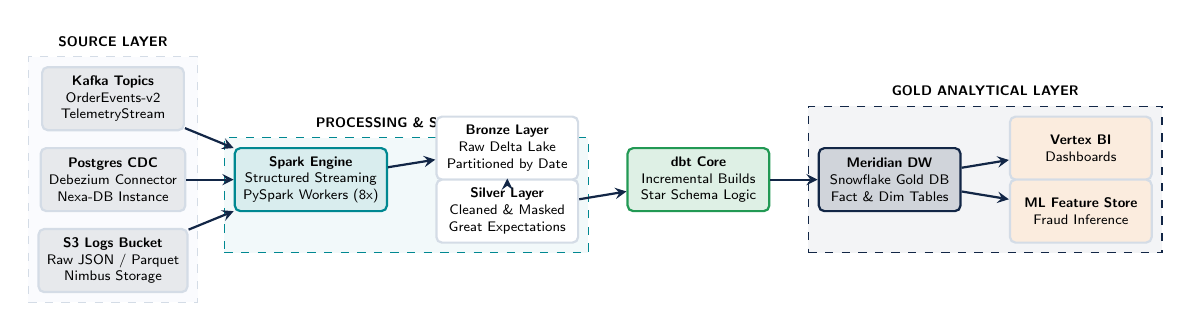
\begin{tikzpicture}[
    node distance=0.6cm and 0.6cm,
    font=\sffamily\tiny,
    boxstyle/.style={rectangle, draw=BorderColor, fill=white, rounded corners=2pt, align=center, inner sep=3pt, font=\sffamily\tiny, minimum width=1.8cm, minimum height=0.8cm, thick},
    arrowstyle/.style={->, >=stealth, thick, PrimaryBlue}
]

    % Layer 1: Sources
    \node (src_kafka) [boxstyle, fill=PrimaryBlue!10] {\textbf{Kafka Topics}\\\tiny OrderEvents-v2\\\tiny TelemetryStream};
    \node (src_cdc) [boxstyle, fill=PrimaryBlue!10, below=0.2cm of src_kafka] {\textbf{Postgres CDC}\\\tiny Debezium Connector\\\tiny Nexa-DB Instance};
    \node (src_s3) [boxstyle, fill=PrimaryBlue!10, below=0.2cm of src_cdc] {\textbf{S3 Logs Bucket}\\\tiny Raw JSON / Parquet\\\tiny Nimbus Storage};

    % Layer 2: Ingestion & Streaming Engine
    \node (spark) [boxstyle, draw=AccentTeal, fill=AccentTeal!15, right=0.6cm of src_cdc] {\textbf{Spark Engine}\\\tiny Structured Streaming\\\tiny PySpark Workers (8x)};

    % Layer 3: Delta Storage (Bronze / Silver)
    \node (bronze) [boxstyle, right=0.6cm of spark, yshift=0.4cm] {\textbf{Bronze Layer}\\\tiny Raw Delta Lake\\\tiny Partitioned by Date};
    \node (silver) [boxstyle, right=0.6cm of spark, yshift=-0.4cm] {\textbf{Silver Layer}\\\tiny Cleaned \& Masked\\\tiny Great Expectations};

    % Layer 4: Transformation (dbt)
    \node (dbt) [boxstyle, draw=SuccessGreen, fill=SuccessGreen!15, right=0.6cm of silver, yshift=0.4cm] {\textbf{dbt Core}\\\tiny Incremental Builds\\\tiny Star Schema Logic};

    % Layer 5: Target Warehouse (Gold)
    \node (snowflake) [boxstyle, draw=PrimaryBlue, fill=PrimaryBlue!20, right=0.6cm of dbt] {\textbf{Meridian DW}\\\tiny Snowflake Gold DB\\\tiny Fact \& Dim Tables};

    % Layer 6: Downstream Consumers
    \node (bi) [boxstyle, fill=WarningAmber!15, right=0.6cm of snowflake, yshift=0.4cm] {\textbf{Vertex BI}\\\tiny Dashboards};
    \node (ml) [boxstyle, fill=WarningAmber!15, right=0.6cm of snowflake, yshift=-0.4cm] {\textbf{ML Feature Store}\\\tiny Fraud Inference};

    % Connections
    \draw [arrowstyle] (src_kafka) -- (spark);
    \draw [arrowstyle] (src_cdc) -- (spark);
    \draw [arrowstyle] (src_s3) -- (spark);

    \draw [arrowstyle] (spark) -- (bronze);
    \draw [arrowstyle] (bronze) -- (silver);
    \draw [arrowstyle] (silver) -- (dbt);
    \draw [arrowstyle] (dbt) -- (snowflake);

    \draw [arrowstyle] (snowflake) -- (bi);
    \draw [arrowstyle] (snowflake) -- (ml);

    % Background Grouping Boxes
    \begin{scope}[on background layer]
        \node [draw=BorderColor, dashed, fill=LightBg!50, fit=(src_kafka) (src_s3), label=above:{\tiny \textbf{SOURCE LAYER}}] {};
        \node [draw=AccentTeal, dashed, fill=AccentTeal!5, fit=(spark) (silver), label=above:{\tiny \textbf{PROCESSING \& STORAGE}}] {};
        \node [draw=PrimaryBlue, dashed, fill=PrimaryBlue!5, fit=(snowflake) (bi) (ml), label=above:{\tiny \textbf{GOLD ANALYTICAL LAYER}}] {};
    \end{scope}

\end{tikzpicture}%
}
\end{center}

\vspace{2pt}

% ==============================================================================
% SECTION 3: DATA WAREHOUSE SCHEMA & DIMENSIONAL MODEL
% ==============================================================================
\section{Data Warehouse Schema \& Dimensional Specification}

The target analytical layer in \textbf{Meridian Snowflake Warehouse} adopts a Kimball Star Schema design optimized for high-throughput aggregation and fast analytical query processing.

\subsection{Gold Fact Table: \texttt{gold\_fact\_orders}}
This table stores transactional order activity enriched with currency conversion and dimension keys.

\vspace{2pt}

\scriptsize
\begin{tabularx}{\textwidth}{@{}p{2.8cm}p{2.2cm}p{1.4cm}p{1.2cm}L@{}}
\toprule
\rowcolor{PrimaryBlue!15}
\textbf{Column Name} & \textbf{Data Type} & \textbf{Constraint} & \textbf{Nullable?} & \textbf{Description \& Transformation Rules} \\
\midrule
\texttt{order\_sk} & \texttt{BIGINT} & PK & No & Surrogate Key (MD5 Hash of \texttt{order\_id} + \texttt{created\_at}). \\
\texttt{order\_id} & \texttt{VARCHAR(64)} & BK & No & Natural Order Identifier from Postgres CDC. \\
\texttt{customer\_sk} & \texttt{INT} & FK & No & Foreign Key matching \texttt{gold\_dim\_customers}. \\
\texttt{product\_sk} & \texttt{INT} & FK & No & Foreign Key matching \texttt{gold\_dim\_products}. \\
\texttt{order\_timestamp\_utc} & \texttt{TIMESTAMP\_NTZ} & -- & No & Event timestamp converted to UTC. Partition key. \\
\texttt{gross\_amount\_usd} & \texttt{NUMBER(12,2)} & -- & No & Raw order total converted to USD at event time rate. \\
\texttt{tax\_amount\_usd} & \texttt{NUMBER(10,2)} & -- & Yes & Calculated tax amount in USD. \\
\texttt{order\_status} & \texttt{VARCHAR(32)} & Check & No & Allowed: \texttt{PENDING, COMPLETED, REFUNDED, CANCELLED}. \\
\texttt{is\_fraud\_flagged} & \texttt{BOOLEAN} & -- & No & Flag derived from ML inference stream. Default: \texttt{FALSE}. \\
\texttt{etl\_inserted\_at} & \texttt{TIMESTAMP\_NTZ} & -- & No & Pipeline processing timestamp for auditing. \\
\bottomrule
\end{tabularx}

\vspace{4pt}

\subsection{Gold Dimension Table: \texttt{gold\_dim\_customers} (SCD Type 2)}
Customer dimension preserving historical state updates (e.g., tier changes, address updates).

\vspace{2pt}

\begin{tabularx}{\textwidth}{@{}p{2.8cm}p{2.2cm}p{1.4cm}p{1.2cm}L@{}}
\toprule
\rowcolor{PrimaryBlue!15}
\textbf{Column Name} & \textbf{Data Type} & \textbf{Constraint} & \textbf{Nullable?} & \textbf{Description \& Business Rules} \\
\midrule
\texttt{customer\_sk} & \texttt{INT} & PK & No & Auto-incrementing Surrogate Key. \\
\texttt{customer\_id} & \texttt{VARCHAR(64)} & BK & No & Unique Customer Natural Identifier. \\
\texttt{customer\_name\_hash} & \texttt{VARCHAR(64)} & PII & No & SHA-256 Hashed Customer Name for anonymity. \\
\texttt{email\_domain} & \texttt{VARCHAR(128)} & -- & Yes & Extracted domain portion of email (e.g., \texttt{nexa.io}). \\
\texttt{account\_tier} & \texttt{VARCHAR(32)} & -- & No & Tiers: \texttt{STANDARD, PREMIUM, ENTERPRISE}. \\
\texttt{country\_code} & \texttt{CHAR(2)} & -- & No & ISO 3166-1 alpha-2 country code. \\
\texttt{effective\_start\_date} & \texttt{DATE} & -- & No & Validity start date for SCD Type 2 record. \\
\texttt{effective\_end\_date} & \texttt{DATE} & -- & Yes & Validity end date (\texttt{NULL} if current active record). \\
\texttt{is\_current} & \texttt{BOOLEAN} & -- & No & \texttt{TRUE} for current record state, \texttt{FALSE} for historical. \\
\bottomrule
\end{tabularx}

\vspace{4pt}

\subsection{Partitioning, Clustering \& Indexing Strategy}
\begin{tcolorbox}[basebox, title=\faDatabase\ Warehouse Optimization Settings]
\scriptsize
\begin{itemize}[leftmargin=1.2em, itemsep=1pt, topsep=1pt]
    \item \textbf{Snowflake Clustering Keys:} \texttt{gold\_fact\_orders} is clustered by \texttt{(order\_timestamp\_utc::DATE, customer\_sk)}. Re-clustering runs automatically on 50 GB threshold deltas.
    \item \textbf{Delta Lake Partitioning:} Bronze/Silver Delta tables are partitioned by \texttt{date=YYYY-MM-DD/hr=HH} to accelerate backfill execution and vacuum cycles.
    \item \textbf{Micro-Partition Pruning:} All dbt incremental models enforce a 3-day lookback filter (\texttt{order\_timestamp\_utc >= CURRENT\_DATE - INTERVAL '3 DAYS'}) to eliminate unnecessary scan overhead.
\end{itemize}
\end{tcolorbox}

% ==============================================================================
% SECTION 4: ETL LOGIC & CODE SPECIFICATIONS
% ==============================================================================
\section{ETL Logic \& Code Specifications}

\subsection{Incremental Data Transformation (dbt Model)}
The following production SQL model executes within dbt to incrementally merge Silver staging records into the \texttt{gold\_fact\_orders} analytical target table.

\vspace{2pt}

\begin{lstlisting}[style=sqlstyle, caption={dbt Model: \texttt{models/gold/gold\_fact\_orders.sql}}]
{{ config(
    materialized='incremental',
    unique_key='order_sk',
    cluster_by=['order_timestamp_utc::DATE', 'customer_sk'],
    incremental_strategy='merge'
) }}

WITH silver_staged AS (
    SELECT 
        MD5(CONCAT(order_id, ':', created_at)) AS order_sk,
        order_id,
        customer_id,
        product_id,
        DATE_TRUNC('second', created_at) AS order_timestamp_utc,
        ROUND(gross_amount * fx_rate_to_usd, 2) AS gross_amount_usd,
        ROUND(tax_amount * fx_rate_to_usd, 2) AS tax_amount_usd,
        UPPER(order_status) AS order_status,
        COALESCE(fraud_score > 0.85, FALSE) AS is_fraud_flagged,
        CURRENT_TIMESTAMP() AS etl_inserted_at
    FROM {{ ref('silver_orders_cleansed') }}
    {% if is_incremental() %}
        -- Incremental processing lookback window to handle late-arriving data
        WHERE created_at >= (SELECT MAX(order_timestamp_utc) - INTERVAL '3 DAYS' FROM {{ this }})
    {% endif %}
),

dim_customers AS (
    SELECT customer_sk, customer_id 
    FROM {{ ref('gold_dim_customers') }} 
    WHERE is_current = TRUE
)

SELECT 
    s.order_sk,
    s.order_id,
    COALESCE(c.customer_sk, -1) AS customer_sk, -- -1 handles unmapped dimensions
    s.product_id AS product_sk,
    s.order_timestamp_utc,
    s.gross_amount_usd,
    s.tax_amount_usd,
    s.order_status,
    s.is_fraud_flagged,
    s.etl_inserted_at
FROM silver_staged s
LEFT JOIN dim_customers c ON s.customer_id = c.customer_id;
\end{lstlisting}

\vspace{3pt}

\subsection{PySpark Ingestion \& PII Sanitization Handler}
The raw streaming engine executes PII hashing and schema validation prior to writing Bronze records.

\vspace{2pt}

\begin{lstlisting}[style=pysparkstyle, caption={PySpark Processor: \texttt{jobs/ingest\_orders\_stream.py}}]
from pyspark.sql import SparkSession
from pyspark.sql.functions import col, sha2, concat_ws, current_timestamp, from_json
from pyspark.sql.types import StructType, StructField, StringType, DoubleType, TimestampType

def process_orders_stream(spark: SparkSession, kafka_bootstrap: str):
    schema = StructType([
        StructField("order_id", StringType(), False),
        StructField("customer_id", StringType(), False),
        StructField("customer_name", StringType(), True),
        StructField("gross_amount", DoubleType(), False),
        StructField("timestamp", StringType(), False)
    ])

    raw_stream = spark.readStream \
        .format("kafka") \
        .option("kafka.bootstrap.servers", kafka_bootstrap) \
        .option("subscribe", "nexa.synapse.orders.v2") \
        .option("startingOffsets", "latest") \
        .load()

    parsed_df = raw_stream \
        .select(from_json(col("value").cast("string"), schema).alias("data")) \
        .select("data.*")

    # Enforce PII Masking: Hash customer_name using SHA-256 with static platform salt
    sanitized_df = parsed_df \
        .withColumn("customer_name_hash", sha2(concat_ws("::", col("customer_name"), col("customer_id")), 256)) \
        .drop("customer_name") \
        .withColumn("ingested_at", current_timestamp())

    query = sanitized_df.writeStream \
        .format("delta") \
        .outputMode("append") \
        .option("checkpointLocation", "s3a://nexa-synapse-checkpoints/orders_v2/") \
        .partitionBy("ingested_at") \
        .start("s3a://nexa-synapse-lake/bronze/orders/")
        
    return query
\end{lstlisting}

% ==============================================================================
% SECTION 5: DATA QUALITY, MONITORING & SLAS
% ==============================================================================
\section{Data Quality Controls, Validation Rules \& SLAs}

Data quality is verified at each pipeline boundary using automated assertions powered by Great Expectations and Soda Core.

\subsection{Automated Validation Matrix}
\vspace{2pt}

\scriptsize
\begin{tabularx}{\textwidth}{@{}l l L L c@{}}
\toprule
\rowcolor{PrimaryBlue!15}
\textbf{Rule ID} & \textbf{Target Field} & \textbf{Assertion Check} & \textbf{Threshold / SLA} & \textbf{Action on Failure} \\
\midrule
\texttt{DQ-ORD-01} & \texttt{order\_id} & Expect column values to never be NULL & 100\% Compliance & Quarantine to DLQ \\
\texttt{DQ-ORD-02} & \texttt{gross\_amount} & Expect value to be strictly positive ($> 0.00$) & 99.99\% Row Pass & Quarantine to DLQ \\
\texttt{DQ-ORD-03} & \texttt{created\_at} & Timestamps within 24h of system time & Max Drift $< 15$ min & Trigger Slack Alert \\
\texttt{DQ-CUST-04} & \texttt{customer\_sk} & Foreign Key integrity matching \texttt{dim\_customers} & $> 99.50\%$ Match & Assign Default \texttt{-1} \\
\texttt{DQ-LAT-05} & End-to-End Stream & Stream ingestion latency from Kafka source & P99 $< 180$ Seconds & Page On-Call DE \\
\bottomrule
\end{tabularx}

\vspace{4pt}

\subsection{Dead Letter Queue (DLQ) \& Error Recovery Protocol}
\begin{tcolorbox}[calloutbox]
\scriptsize \textcolor{PrimaryBlue}{\textbf{\faLock\ Dead Letter Queue (DLQ) Execution Workflow:}} \\[2pt]
When a record violates critical assertions (\texttt{DQ-ORD-01} or \texttt{DQ-ORD-02}), it is routed to the S3 quarantine location \texttt{s3://nexa-synapse-dlq/orders/}. 
\begin{enumerate}[leftmargin=1.5em, itemsep=1pt, topsep=1pt]
    \item \textbf{Alert Notification:} Prefect fires an automated incident payload to PagerDuty (\texttt{\#alerts-data-ops}).
    \item \textbf{Inspection \& Patching:} Engineers inspect quarantine payloads using the Nexa DataOps CLI Tool:
    \begin{center}
    \texttt{\scriptsize nexa-dataops dlq inspect --pipeline PL-2026-SYN-088 --date 2026-07-24}
    \end{center}
    \item \textbf{Replay Trigger:} Fixed records are re-published to the replay Kafka topic \texttt{nexa.synapse.orders.replay} for re-processing.
\end{enumerate}
\end{tcolorbox}

% ==============================================================================
% SECTION 6: SECURITY, GOVERNANCE & RUNBOOK
% ==============================================================================
\section{Security, Governance \& Operational Runbook}

\subsection{Access Control Matrix (RBAC)}
Data access in \textbf{Meridian Warehouse} adheres to the principle of least privilege using Snowflake role hierarchies.

\vspace{2pt}

\scriptsize
\begin{tabularx}{\textwidth}{@{}l L L L@{}}
\toprule
\rowcolor{PrimaryBlue!15}
\textbf{Role Name} & \textbf{Bronze Layer} & \textbf{Silver Layer} & \textbf{Gold Layer Access} \\
\midrule
\texttt{NEXA\_DATAOPS\_ADMIN} & FULL ACCESS & FULL ACCESS & FULL ACCESS (DDL + DML) \\
\texttt{SYNAPSE\_TRANSFORMER} & READ ONLY & READ + WRITE & READ + WRITE (dbt Executor) \\
\texttt{VERTEX\_BI\_ANALYST} & NO ACCESS & NO ACCESS & READ ONLY (PII Masked Columns) \\
\texttt{MERIDIAN\_AUDITOR} & NO ACCESS & READ (Audit Logs) & READ ONLY (Compliance Views) \\
\bottomrule
\end{tabularx}

\vspace{4pt}

\subsection{Operational Runbook \& Incident Recovery Commands}
The following standard operating procedure (SOP) applies when recovering from upstream Kafka ingestion halts or performing manual data backfills.

\vspace{2pt}

\begin{tcolorbox}[basebox, title=\faCogs\ DataOps Operational Backfill Procedure]
\scriptsize
\textbf{Scenario:} Source system outage required a 48-hour data backfill for period \texttt{2026-07-20} to \texttt{2026-07-22}.

\begin{enumerate}[leftmargin=1.5em, itemsep=2pt]
    \item \textbf{Pause Real-Time Orchestrator:}
    Disable the Prefect schedule to avoid concurrent writing conflicts:
    \begin{center}
    \texttt{\scriptsize prefect deployment pause "synapse-etl-pipeline/production-stream"}
    \end{center}

    \item \textbf{Execute Backfill PySpark Job:}
    Submit the backfill Spark job targeting the specific historical date partition range:
    \begin{center}
    \texttt{\scriptsize spark-submit --master k8s://https://k8s.nexa.internal:6443 \textbackslash{}} \\
    \texttt{\scriptsize \quad --deploy-mode cluster --num-executors 16 --executor-memory 8G \textbackslash{}} \\
    \texttt{\scriptsize \quad jobs/backfill\_orders.py --start-date 2026-07-20 --end-date 2026-07-22}
    \end{center}

    \item \textbf{Re-run dbt Incremental Models with Full Refresh Filter:}
    \begin{center}
    \texttt{\scriptsize dbt run --select path:models/gold/gold\_fact\_orders.sql --vars '\{"backfill": true, "start\_date": "2026-07-20"\}'}
    \end{center}

    \item \textbf{Run Data Reconciliation Suite \& Unpause:}
    Verify row counts match source Postgres CDC offsets, then resume real-time deployment:
    \begin{center}
    \texttt{\scriptsize dbt test --select test\_type:singular \&\& prefect deployment resume "synapse-etl-pipeline/production-stream"}
    \end{center}
\end{enumerate}
\end{tcolorbox}

\vspace{4pt}

\begin{center}
    \textcolor{SubtleGray}{\small --- \textbf{END OF TECHNICAL SPECIFICATION} \ \textbar\ \ Nexa Data Platform Architecture Board ---}
\end{center}

\end{document}
